%%%%%%%%%%%%%%%%%%%%%%%%%%%%%%%%%%%%%%%%%%%%%%%%%%%%%%%%%%%%%%%%%%%%%%%%%%
%
%    JWST_sci_template.tex  (use only for JWST General Observer and Archival Research proposals)
%
%
%
%    JAMES WEBB SPACE TELESCOPE
%    OBSERVING PROPOSAL TEMPLATE
%    FOR CYCLE 1 (2017)
%
%    Version 1.0 September 2017.
%
%    Guidelines and assistance
%    =========================
%     Cycle 1 Announcement Web Page:
%
%         https://jwst-docs.stsci.edu/display/JSP/JWST+Cycle+1+Proposal+Opportunities
%
%    Please contact the JWST Help Desk if you need assistance with any
%    aspect of your proposal:
%    	    http://jwsthelp.stsci.edu
%
%
%
%%%%%%%%%%%%%%%%%%%%%%%%%%%%%%%%%%%%%%%%%%%%%%%%%%%%%%%%%%%%%%%%%%%%%%%%%%%

% The template begins here. Please do not modify the font size from 12 point.

\documentclass[12pt]{article}
\usepackage{jwstproposaltemplate}
\usepackage{hyperref}
\usepackage{graphicx}
\usepackage{floatrow}
\usepackage{sidecap}
\sidecaptionvpos{figure}{t}


\usepackage{caption}
\captionsetup[figure]{labelfont=bf, font=footnotesize}
\captionsetup[table]{labelfont=bf, font=footnotesize}

\usepackage{natbib}
\bibliographystyle{mnras}

\setlength{\textfloatsep}{5pt}
\usepackage{color}

\newcommand{\todo}[1]{\textbf{**TODO: \textcolor{red}{#1}**}}


\begin{document}

%   1. SCIENTIFIC JUSTIFICATION
%       (see https://jwst-docs.stsci.edu/jwst-opportunities-and-policies/jwst-call-for-proposals-for-cycle-1/jwst-cycle-1-proposal-preparation)
%
%






\todo{Abstract. Delete later.}

Pure parallel opportunities on \emph{Webb} offer the opportunity, \emph{almost at no extra telescope time cost}, to build up a large amount of public NIRCam imaging. We propose to exploit the longest available parallel opportunities to build up $\sim 150\ {\rm arcmin^2}$ of deep (F200W$=29-29.5$, $5\sigma$ point-source) multi-band NIRCam imaging data. This proposal - the Public Ultradeep Pure Parallel Imaging Extragalactic Survey (PUPPIES) - will push at least $0.5$ mag deeper than the public Cosmic Evolution Early Release Science Survey and will cover a comparable area. The core objective of PUPPIES is the identification of faint galaxies at $z>9$. PUPPIES will provide the first meaningful constraints on the faint-end slope and normalisation of luminosity function. Through its  multi-band observations WAFLS will probe the stellar populations and dust content of these galaxies providing insight to their formation and evolution during this critical period of the Unvierse's history.



\clearpage

\justification          % Do not delete this command.

\section{Background}

One of the scientific cornerstones of the James Webb Space Telescope is to determine how the first stars and galaxies formed in the early Universe. As such, Webb's capability will reveal how the first galaxies assembled, the nature of the sources that reionised the Universe, and how the diverse galaxy population we can study at $z \sim 3-6$ was established at higher redshifts.  We can observe galaxies up to

The Hubble Space Telescope has spent several 1000s of orbits over two decades to solve the problem of evolution/formation of galaxies which existed when the universe was 500 Myr old until today. This has led to fantastic results on early galaxy formation and cosmic dawn at redshifts $z \sim 6-10$. Yet we know from these observations that we have not yet reached the very first epoch of galaxies due to the limited depth in the near infrared provided by Hubble. This is a problem that will necessarily receive intense attention with JWST from both GTO and GO observations, and because this problem is observationally so difficult it will require clever strategies and multiple data collecting methods.

The past near-decade of wide and deep surveys with the {\it Hubble Space Telescope’s} ({\it HST}) Wide Field Camera 3 (WFC3) has begun the process of exploration of this key epoch in the Universe’s history.  Wide and deep surveys with WFC3 over the Hubble Ultra Deep Field (HUDF; Beckwith et al. 2006; Bouwens et al.\ 2010; DUNLOP+), Cosmic Assembly Near-Infrared Deep Extragalactic Legacy Survey (CANDELS; Grogin et al.\ 2011; Koekemoer et al.\ 2011), and the Frontier Fields project (Lotz et al. 2017) enabled the construction of the first large samples of galaxies at $z>7$.  

Among the discoveries made with these data to date include: 1) While the faint-end slope of the UV luminosity function steepens significantly at $z>7$, the bright-end shows less evolution (e.g., Bouwens et al.\ 2015; Finkelstein et al.\ 2015); 2) The abundance of galaxies, when integrated to very faint limits now provided seemingly feasible from lensing studies (e.g., Atek et al.\ 2015; Livermore et al.\ 2017) imply that galaxies produce enough photons to complete reionization by $z\sim$ 6, though only if the ionizing photon escape fraction is $\gtrsim$10\% (REFERENCES); 3) Bright/massive galaxies appear modestly dusty, showing an early onset of chemical enrichment (Finkelstein et al.\ 2012; Bouwens et al.\ 2014, UPDATE REFERENCES), and 4) Some bright/massive galaxies exist out to at least $z \sim$ 10 (e.g. Oesch et al.\ 2016; add in reference to RELICS).

Little is however known concerning the galaxy population at $z > 9$ beyond the discovery of a few candidate galaxies.  While some observational studies of the evolution of the galaxy population imply a dramatic decline in the UV luminosity density (and by extension, star-formation rate density) at $z >$ 9 (e.g., Bouwens et al.\ 2015; Oesch et al.\ 2018), others see no such decline (e.g., Coe et al.\ 2013; McLeod et al.\ 2016), and the discovery of an unexpectedly luminous galaxy at $z >$ 10 (Oesch et al.\ 2016) points towards potentially significant amounts of star-formation activity remaining to be discovered in this early epoch of galaxy formation.    The high stellar masses of galaxies at $z \sim 7$ and the fact that the the UV continuum shows no signs of Pop III stars (Bhatawdekar et al. 2020), strongly suggests that the first epoch of galaxy formation has yet to be found.

Predictions of the properties of galaxies at $z > 9$ also varies in different simulations (see left-panel of Fig. 4). It is clear however that those simulations that account for the evolution of the physical conditions promoting star formation, including its dependence on gas density, show that {\it Webb}-detectable galaxies exist  at $z >$ 9 (e.g., Yung et al.\ 2018).  A key question for the opening cycles of {\it Webb} is this — is there significant star-formation activity at  $9<z<12$, or does the limiting redshift of {\it HST} just happen to coincide with the time when the universe began its first large-scale episode of star formation?

The planned GTO/ERS programs, in particular the Cosmic Evolution Early Release Science (CEERS), the Webb Medium Deep Fields (WMDF), and the JWST Advanced Deep Survey (JADES), will begin the process of obtaining stronger constraints at $z>9$.   However, while all of these programs will likely find $z > 9$ galaxies, they are subject to strong cosmic variance as well as limited areas probed.  JADES will likely yield more systems at these redshifts, but the observations will be spread over the first 3 cycles, with the full data-set potentially not becoming public until 4 years after launch. Hence we propose the \textbf{Public Ultradeep Pure Parallel Imaging Extragalactic survey (PUPPIES)} that will generate a dataset of similar depth to JADES medium survey but will be publicly available in Webb's cycle 1 to the entire astronomical community. 


{\bf The Public Ultradeep Pure Parallel Imaging Extragalactic Survey (PUPPIES) is a pure parallel opportunity to rapidly build up a large area of very-deep F200W$>29$ public multi-band NIRCam imaging.}  The use of pure parallel imaging to search for the most massive and bright systems has proven to be an important aspect for finding distant galaxies with Hubble in programs such as HIPPIES (Yan et al., 2011) and BoRG (Trenti et al., 2011), allowing for the bright end of the luminossity function at $z > 7$ to be sudied in complement to the fainter galaxies found in the pointed observations of the deep fields.  With JWST a similar strategy of mixing parallel observations with pointed ones will be a powerful way to search for and find the rarer brighter systems that will be more amenable to follow up observations.   PUPPIES will obtain deep multi-band near-IR public imaging using NIRCam. PUPPIES will survey an area similar or slightly larger than the public CEERS dataset but will reach 0.25-0.5 mag deeper yielding 4-5x more galaxies at $z > 9$ placing the first meaningful constraints on the number of $z > 11$ galaxies (CEERS=2, PUPPIES=10).

Our program will address a host of issues, including the number of early $z > 9$ galaxies, their properties, including their stelalr populations, their structure and sizes and the distributions of these quantities.  These are all important features for solving the very early formation of galaxies that will be a public dataset to suplmenet the deep GTO imaging programs.

\section{Science Goals}

\noindent In this section we enumerate the various science goals of PUPPIES and what we will learn about the early galaxy population through our analyses.

This includes the following science topics:

\begin{enumerate}
\item The robust identification of $\sim 100$ star forming galaxies across the early EoR ($9<z<11$).
\item Cosmic variance minimised constraints on the faint-end of the $9<z<11$ UV luminosity function. 
\item The measurement of the physical properties of the faint $9<z<11$ galaxies including their star formation rates, stellar masses, dust attenuation, and morphologies. 
\end{enumerate}

While focused on the distant Universe PUPPIES will provide an invaluable immediately public legacy resource for answering a range of other science questions, including questions about stellar populations in our own Galaxy. For example, PUPPIES will enable the discovery and typing of low-mass stars and sub-stellar objects throughout the disk and halo of the Milky Way. When we combine PUPPIES with optical observations we will be able to measure accurate stellar masses and star formation rates across cosmic history, reaching down to $M_{\star}\sim 10^{8}\,{\rm M_{\odot}}$ at $z=2$.


\subsection*{\bf UV Luminosity Functions at $z > 9$}\label{sec:UVLF}

A primary goal for JWST is placing constraints on the UV luminosity function across the epoch of reionization and Beyond. When observing galaxies at the highest redshifts we are interested in first of all in finding and characterizing galaxies which exist at these early epochs.  The most straightforward way of doing this is using Ultra-Violet (UV) luminosity function of galaxies, which gives the number densities of galaxies at different UV luminosities, and is the simplest measure of galaxies at these redshifts that requires the least amount of assumptions.  Furthermore, the rest-frame ultraviolet luminosity function, as well as the stellar mass function, will provide us answers to fundamental questions about the way that the first galaxies and stars formed.

Many different physical processes are responsible for the formation of the first galaxies, and thus the creation of UV light, including properties such as the metallicity of the gas and stars,  dust, feedback, the density of gas, as well as magnetic fields.    The predictions for the formation of these first galaxies can vary significantly depending on the  assumptions which go into models.  For example, although the lack of metals in early star formation means that gas cooling will be less efficient, and take longer to occur, this could potentially be counterbalanced by the more rapid formation time resulting from a higher gas density.  The luminosity function is a powerful approach for understanding this issue. With PUPPIES combines with deep programs such as JADES and CEERS we will place strong constraints on the bright- as well as the faint-end of the UV LF.   By comparing with models this will reveal important information about the efficiency of galaxy and star formation at the earliest times in the universe.
 
Currently there are inconsistencies, and large uncertainties, in the best available measurements of galaxy number densities and luminosity functions at $z > 6$.  Based on the deepest existing Hubble data it is intriguing that there is an apparent step decline of the number of galaxies at the highest redshifts, $z \sim 6-11$ (e.g., Ellis et al. 2012; Schenker et al. 2012; Bouwens et al. 2016). Based on extrapolating the UV luminosity function at lower redshifts, we should have found more systems at $z \sim 9-11$ than the candidates discovered in the deepest HST data (e.g., Oesch et al. 2013).  However, deep HST imaging of lensing clusters in the CLASH and HFF clusters have found a significant number of $z>6$ candidates (e.g., Atek et al. 2014; Monna et al. 2014; Vanzella et al. 2014; update).  This includes several lensed candidates at $z\sim 9$ behind the HFFs (e.g., Laporte et al. 2014; Schmidt et al. 2014; Zitrin et al. 2014).   Understanding this possible inconsistency, and minimizing the role of cosmic variance requires deeper and larger area data which PUPPIES will provide.

Overall, the observed luminosity function of galaxies encodes both the  detailed physics of star formation in addition to the effect of dust attenuation. From a theory perspective both of these are sufficiently uncertain, particularly in the early Universe, that different modelling approaches, despite yielding similar results at low-redshift, diverge at high-redshift. This is demonstrated in Figure \ref{fig:CN} where we show the expected cumulative number of galaxies expected in PUPPIES for a range of models. This wide variation demonstrates that the study of galaxies during this epoch has a great potential to inform our understanding of galaxy formation and evolution in the early Universe.


% THIS TEXT IS TAKEN FROM ANOTHER PROPOSAL IN PREP - IT SHARES SOME COIs SO I FEEL ITS FINE AS A REFERENCE

% The first 500 Myr of galaxy evolution (z>10) was a transformative period in our Universe, as the first galaxies began to coalesce, enriching and ionizing their environments, forever altering the course of subsequent gas accretion and star formation. While deep and wide surveys with HST (e.g., HUDF [PI Illingworth], CANDELS [PIs Faber & Ferguson], Hubble Frontier Fields [PI Lotz]) led to the discovery of ∼1000 galaxy candidates at 6< z <8, Hubble has only scratched the surface at z>9, with just a handful of z ∼9–11 tenuous (e.g., <10σ significance in 1–2 imaging bands) candidates [27, 4]. Pushing HST’s limits has led to a tension in published observational results. While there is agreement that the observable (MUV < −17) cosmic SFR density smoothly declines from z = 4 to 8 [e.g., 14, 6], some [e.g., 27] find evidence for an accelerated decline at z > 8, while others [e.g., 25, 12] find evidence for a continued smooth decline to earlier times. The absence of robust observational constraints leaves theoretical models completely unconstrained at z >9 (Figure 2), where differences in their physical star-formation and feedback prescriptions result in a wide range of predictions for the abundance of galaxies during this epoch. This leads to enormous uncertainty on plausible timelines for the reionization of the intergalactic medium (IGM), where models which follow the steep SFR density evolution are consistent with a slow beginning and rapid completetion, while those which follow the shallow SFR evolution find an earlier beginning and more smooth evolution of the reionization process [e.g. 31, 15].
% Robust observational constraints are needed to distinguish between these competing models. This is possible with JWST/NIRCam as its sensitivity over 1 − 5μm allows the measurement of at least two colors over 8 < z < 20, and was designed to go deep, hunting these first galaxies. However, the planned public Early Release Science programs fall short of what is needed to detect these objects. 




\begin{figure}[h!]
    \centering
    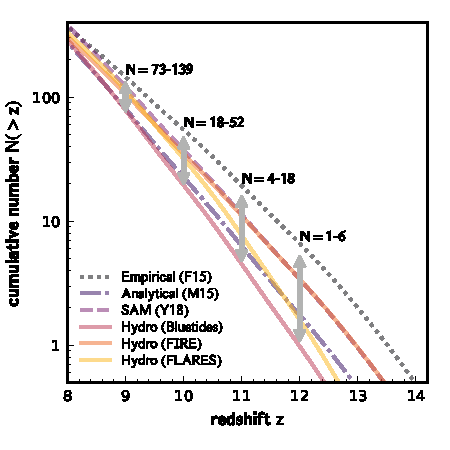
\includegraphics[width=0.49\textwidth]{figs/CN_models.pdf}
    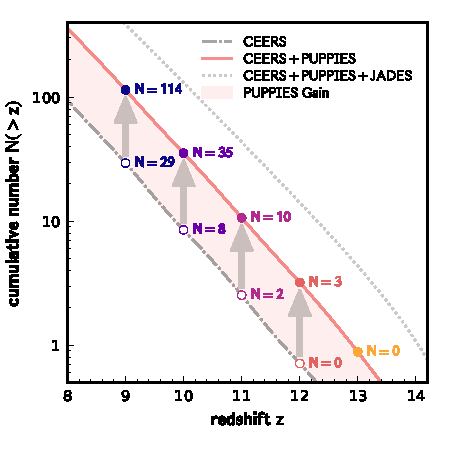
\includegraphics[width=0.49\textwidth]{figs/CN_surveys.pdf}
    \vspace{-5mm}
    \caption{\emph{\underline{Left:}} The cumulative number of galaxies predicted to be accessible to PUPPIES and CEERS for a range of different empirical extrapolations and theoretical models. \textbf{The expected number of galaxies at $z>9$ is uncertain demonstrating the constraining power of PUPPIES. PUPPIES will identify $70-140$ galaxies at $z>9$ and $4-18$ at $z>11$.} \emph{\underline{Right:}} The cumulative number of sources predicted to observable to CEERS, CEERS+PUPPIES, and CEERS+PUPPIES+JADES. \textbf{PUPPIES will boost the number of galaxies at $z>9$ ($z>11$) by a factor of $4$ (5) compared to CEERS alone}. }
    \label{fig:CN}
\end{figure}


\begin{figure}[h!]
    \centering
    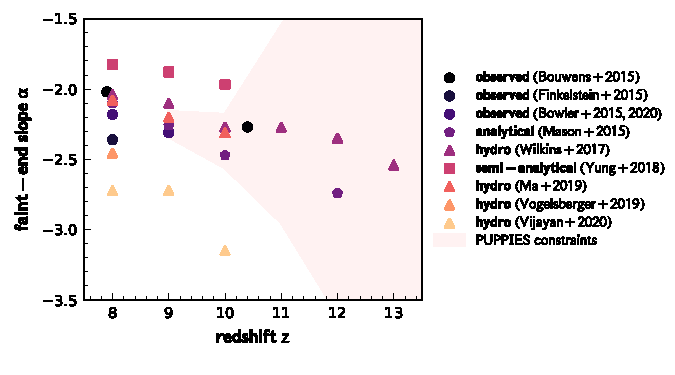
\includegraphics[width=0.8\textwidth]{figs/alpha.pdf}
    \vspace{-5mm}
    \caption{Current observational constraints and theoretical predictions for the faint-end slope $\alpha$ of the luminosity function at $z\ge 8$. \textbf{The faint-end slope of the luminosity function $\alpha$ at $z=8-13$ is highly uncertain.}}
    \label{fig:alpha}
\end{figure}




\begin{SCfigure}
    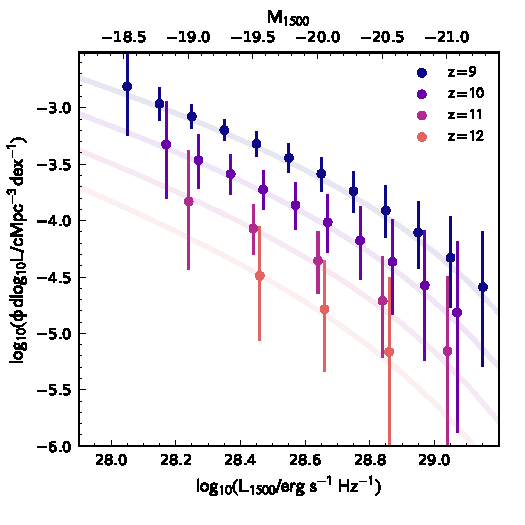
\includegraphics[width=0.6\textwidth]{figs/LF_evo.pdf}
      \caption{\protect\rule{0ex}{10ex} Predicted constraints on the UV luminosity function from PUPPIES at $z=9\to 12$ assuming the Yung et al. (2018) semi-analytical model. \textbf{PUPPIES will enable the first robust constraints on the UV luminosity function at $z>11$.}}
      \vspace{-5mm}
\end{SCfigure}

\todo{What has been done and how will PUPPIES change things?}
\todo{Should we mention Hubble constraints? - I feel we're not fighting Hubble but other Webb programmes.}

While the planned GTO/ERS programmes will begin the process of obtaining stronger constraints at $z>9$ the relatively small areas probed by these programs limits the number of bright galaxies. This limits our ability to constrain the bright-end of the LF, critical to characterise its overall shape. Compounding the small number of sources is the fact that these programmes, as predominantly contiguous surveys, will suffer from cosmic variance increasing the uncertainty on the number of galaxies by $\approx 1.5-2\times$ compared to the statistical uncertainty alone\cite{2020MNRAS.499.2401T}\cite{2020MNRAS.496..754B}\cite{2008ApJ...676..767T}. 

[{\bf paragraph below needs to be updated for PUPPIES}]

The wide area and pure parallel nature of PUPPIES addresses these issues. The WAFLS strategy is tuned to probe $M^{\star}$ ($M_{1500}=-20\ -\ 21$) galaxies at $9<z<11$ yielding roughly uniform number of galaxies per mag at F277W$27.5-29.5$ ($-21<M_{1500}<-18$) when combined with JADES and CEERS. Figure \ref{fig:CV} shows both the predicted number of sources and the total variance compared to the expected statistical variance for WAFLS, CEERS, and JADES. WAFLS yields not only $3\times$ as many galaxies as JADES+CEERS at F277W$<28.25$ but the resulting total uncertainty is virtually cosmic variance mitigated resulting in an even stronger gain. In Figure \ref{fig:LF} we show the resulting constraints on the $9.5<z<10.5$ LF from CEERS+JADES both with and without WAFLS. This highlights the strong improvement, particularly at $-21<M_{1500}<-20$ where $M^{\star}$ is expected to lie. The addition of WAFLS provides roughly uniform sampling of the LF over and reduces the uncertainty on both the parameters by around a factor of $2-3$. As shown in the right-hand panel WAFLS, when combined with CEERS and JADES, is able to discriminate between many current models. 








% THIS TEXT IS TAKEN FROM ANOTHER PROPOSAL IN PREP - IT SHARES SOME COIs SO I FEEL ITS FINE AS A REFERENCE

% 1.1: Physical Processes Regulating the Emergence of the First Galaxies
% The shape of the rest-frame UV luminosity function constrains the relative importance of the physical processes governing the conversion of gas into stars. These processes depends on numerous factors, including density, metallicity, magnetic field strength, turbulence, and a variety of feedback mechanisms. At the highest redshifts we have almost no empirical constraints on these processes, though theoretical predictions for galaxies in this era are beginning to emerge [e.g., 24, 16, 35, 39, 2]. However, these models use different prescriptions for the physics regulating the conversion of gas into stars, resulting in a wide range of predicted z > 10 luminosity functions. For example, Behroozi et al. [2] adopt an ansatz that galaxy specific SFRs (SFR per unit stellar mass) follow their halo’s specific mass accretion rate, reproducing the observed SFR density evolution at z <8. When extrapolated to even earlier times, it predicts a relatively shallow evolution at 8 < z < 15, with very bullish predictions for JWST surveys.
% Models that attempt to include the detailed physics of molecule formation, star forma- tion, and stellar feedback generally make more bearish predictions [e.g., 16, 35, 39], though their predictions differ dramatically at extreme redshifts (z > 8).
% Figure 2 shows the predicted UV luminosity functions from these models at z = 10 (top-
% middle) and z = 12 (top-right). At z =10 there are noticeable differences in the normalization (∆φ∗ ∼ 1 dex) and faint-end slope (∆α ∼ 0.5). This becomes even more evident at z = 12, where the models span ≥ 1 dex across all luminosities, leading to >∼2 dex variations in the normalization φ∗ and nearly 1 dex in the faint-end slope α. We show predictions for the constraints achievable with WDEEP (see Technical Justification for details), which begin to distinguish between these models at MUV = −17.5 (the ∼10σ limit at z =10).
% Why is there such disagreement in these models? As cosmological simulations can-
% not come close to resolving the formation of individual stars, they must assume many key
% physical relationships. Two in particular regulate the shape and normalization of the UV
% luminosity function at high redshift: the star-formation law (or star formation efficiency
% as a function of cold gas surface density), and the prescription for stellar feedback. Yung
% et al. [39] explored these physical processes using a semi-analytic model (SAM), exploring
% how modifications to these relationships altered the UV luminosity function, shown in the
% bottom panel of Figure 2. The purple shading shows the difference in luminosity func-
% tion predictions between assuming a linear relationship between molecular gas density and  ̇
% that SFRD scales as molecular gas density squared Σ∗ ∝ (ΣH2 )2 above a critical H2 surface density (upper envelope). These changes result in strong differences in the bright-end of the ̇UV luminosity function, where medium-depth wide-field programs such as CEERS will place constraints, but little change in the faint-end.

% However, Yung et al. [39] found that stellar feedback strongly influences star formation in low-mass halos, with significant changes in the predicted abundances of faint galaxies. They parameterized this with a stellar feedback relation slope (αrh) which characterizes the dependence of the mass loading factor of cold gas ejected by stellar feedback on the halo circular velocity. Yung et al. [39] found that changing αrh can change the number density of the lowest-mass observable galaxies (∼108M⊙; MUV ∼ −18 at z = 10) by up to 1 dex. The red shaded region in Figure 2 illustrates the range of luminosity function predictions from Yung et al. [39] when changing αrh = 2.0 (top) to 3.6 (bottom). The data points show the precision on the luminosity function measured by CEERS (green) and WDEEP (blue) for Yung et al’s fiducial model (αrh = 2.4). Our predicted WDEEP constraints have uncertainties which are ∼7× smaller than this range in models.
% By robustly identifying galaxies to m > 30, WDEEP will provide the first meaningful constraints on the stellar feedback physics in extremely early galaxies. Constraining the luminosity function to this precision will allow a robust determination of the observed SFR density to z = 12, distinguishing between the wide range of models shown in Figure 2. Finally, by constraining whether the SFR density evolves shallowly or steeply, WDEEP will provide significant constraints on models of reionization.

% As we discover galaxies closer and closer
% to the Big Bang, we will eventually wit-
% ness the periods during which galaxies
% have formed no more than a few gen-
% erations of stars, characterized by ex-
% tremely low metallicities. While pre-
% vious generations of simulations im-
% plied that discovering entire pockets
% of metal-free star-formation was possi-
% ble [so-called “Population III” galaxies;
% e.g. 32], more recent simulations pre-
% dict that Pop III star formation in early
% mini-halos at z ∼ 15–20 was likely very
% efficient at polluting the IGM with met-
% als, and so we might never expect to see
% metal-free star formation [e.g., 18, 17].
% The consequences for subsequent star-
% formation are critical — if all dense gas
% in the universe is rapidly enriched beyond the critical metallicity (Z ∼ 10−4 Z⊙), both the stellar initial mass function and stellar photospheric temperatures will likely not be dramat- ically different than that seen in low-metallicity environments in the early universe. If the opposite is true, and fairly massive metal-free stars can form down to even z ∼ 10, it will provide a distinct boost in the typical hardness of stellar spectra, with consequences on the ability of stellar light to reionize the IGM.
% Constraints on the typical metallicities of early galaxies are thus of intense interest. A straightforward measure of the physical properties of the stars is available via the UV spectral slope β; fλ ∝ λβ [9], which can be measured via broadband colors, with β < −3 a typical threshold for near-metal-free stellar populations. Observations with HST at z < 10 found no strong evidence for β < −2.5, thus the presently observable galaxies are consistent with somewhat low, but non-zero, metallicities, without much dust obscuration in the lowest mass galaxies [13, 10, 5, 34]. Our proposed NIRCam observations will measure four (three) rest-UV colors for galaxies at z ∼ 10 (12), allowing us to constrain the nature of their stellar populations. Simulations at our proposed depths show that with these multiple colors we can recover β with minimal bias and σβ = 0.2 to z > 13. Finally, our observations will improve measures of galaxies at z = 6–8, currently restricted to just one or two colors, measuring β with five colors.

%At the highest redshifts, where only the rest-frame UV
%(dominated by emission from the most massive, young
%but short-lived hot stars) is currently accessible at high
%resolution imaging, one of the few characteristics of the
%physical properties of galaxies available is the UV colour,
%which is sensitive to star formation, dust and metallicity. The inspection of dust and metallicity in the early galaxies can be carried out through the measurement of the UV spectral slope, $\beta$, such that the UV spectral energy distribution has the form $f_{\lambda}\propto\lambda^{\beta}$ (e.g., calzetti et al 1994.) Notably, values of $\beta\sim-3$ suggest the presence of young, extremely metal-poor stellar population. Observations so far show that this slope, $\beta$, is consistent with a very low, but still non-zero metallicity, for low luminous galaxies at z < 10, yet the results overall are not entirely consistent (e.g., Dunlop et al. 2013; Bouwens et al. 2014; ; Finkelstein et al 2012; Wilkins et al 2016). Futhermore, these UV slopes are only found at $M_{\mathrm{UV}}<-17$. This is crucial as models predict that galaxies with $\beta\sim-3$ only exist at $\mathrm{M_{UV}>-17}$ \citep{Dunlop2013}. The HFF data offered the first insights into the rest-frame UV colours of galaxies in a wide magnitude range $-22<\mathrm{M_{UV}<-13}$, finding no evidence for extreme stellar populations or Pop III stars at z > 6 (Bhatawdekar et al. 2020).






\subsection*{Stellar populations and early enrichment}\label{sec:properties}


As we look back towards the Big Bang the galaxies we discover become increasingly deficient in metals and dust. 

Key to identifying both extremely low-metallicity galaxies and constraining the contribution of obscured star formation to the total are observations of the UV continuum slope $\beta$ where $f_{\lambda}\propto\lambda^{\beta}$. 

Very blue ($\beta -3$) slopes are only realised for extremely metal poor and dust free stellar populations.

PUPPIES 

and potentially at $z<8$ 








This will allow us, for the first time, to \underline{consistently} $\beta$ across the entire reionisation epoch $6<z<12$ of galaxies providing the bulk of the ionising photon output of the Universe. 

In addition to $\beta$ PUPPIES will also obtain F444W photometry probing beyond the Balmer-break at $9<z<11$. Photometry beyond the Balmer-break is essential - see technical justification - to measure stellar masses, and thus constrain the galaxy stellar mass function and stellar mass - specific star formation rate relation. 





 These properties include dust attenuation, stellar metallicity, star formation history, and ionising photon escape fraction \cite{2013MNRAS.430.2885W}. In particularly blue slopes ($\beta\simeq -3$) are indicative of the presence a young, low-metallicity, stellar population. While measurements of $\beta$ are available at $z\approx 7$ with {\em Hubble} these are typically measured with single colors over a relatively short wavelength baseline, leading to large uncertainties and biases. While it is possible to measure $\beta$'s at $z\approx 10$ by combining {\em Hubble} and {\em Spitzer} observations \cite{2016MNRAS.455..659W}, these rely on the significantly shallower {\em Spitzer} imaging and have larger uncertainties. Our filter strategy with PUPPIES (see Figure \ref{fig:SED}) will enable the consistent measurement of $\beta$ at $9<z<11$ over the entire rest-frame UV continuum. 







\subsection{\bf Resolved Structures}

The resolved structures of galaxies encodes information about their structural properties and formation histories and are key observables that can be compared to galaxy formation models.  However we know next to nothing about these properties of $z > 9$ galaxies even though this type of analysis has proven very benefical at lower redshifts (e.g., Mortlock et al. 2013).  Morphologies are also an important assumption used in the measurement of the luminosity function (reference) and only by simultaneously modelling the morphologies, redshifts, and fluxes is it possible to self-consistently measure the luminosity function and its uncertainties. Leveraging NIRCam's resolution we will provide sizes and morphologies of $9<z<11$ galaxies across the rest-frame UV ($0.1-0.4\mu$m). \todo{Maybe we should make a plot comparing the predicted size of galaxies to the NIRCam pixel scale and PSF?}  As can be seen in Figure~XX we will be able too determine stuctural properties of these galaxies just past the balmer break.

What we do know is that massive galaxies at $z < 6$ are often very compact and evolve into red nuggets that have extenguished their star formation a few Gyr after the big bang.  What we do not know is how this occurred.  This is such that these quenched passive ‘red nuggets’ are up to five times smaller at z~3-6 than galaxies of the same mass today.  Since these are certainly the progenitors of modern massive galaxies, studying the ancestors of these compact passive/red galaxies at even higher redshifts is crucial for deciphering their origin.   What we can answer this PUPPIES data is how these early galaxies first formed -- were they large star forming systems that later become compact through some process (Barro et al. 2013; Tacchella et al. 2016)? Or, did these systems formed as compact systems to begin with (e.g., Lilly & Carollo 2016)?   Because our parallel imaging will find the most massive systems, and therefore the progentiors of these passive galaxies, we can answer this question by measuring the sizes of these galaxies.

Related to this is that it is clear that merging activity is very important for distant galaxies up to $z \sim 6$ and likely is even more important at higher redshifts.  The evolution of the density of matter at these early phases of the universe goes as $\sim (1+z)^{3}$, implying that galaxies at $z > 9$ were in a more denser universe than at later times. This implies that the merger rate should be even higher than what we can measure at $z < 6$ with HST.  Duncan et al. (2019) showed that $\sim 40$\% of massive galaxies at $z \sim 6$ are in pairs, with an inferred merger rate of $\sim 10$ mergers Gyr$^{-1}$.  In hierarchical models of galaxy formation these galaxies should be undergone intense merging, which is something that we are directly detect. It is ideal to test this with massive systems which are the easiest observational to find mergers for, given that the secondary system in a pair can be over a magnitude fainter for major mergers.  If we extrapolate the merger fraction history that we can measure at $z > 6$ we find that there should be over 60\% of galaxies in pairs.  This is also a prediction of models such as Illustris and Eagle, which we can test at this high density region of the early universe.  Given that we will detect XX galaxies, our shot noise will produce a merger fraction which is less than 10\% on this measurement.  

\begin{SCfigure}
    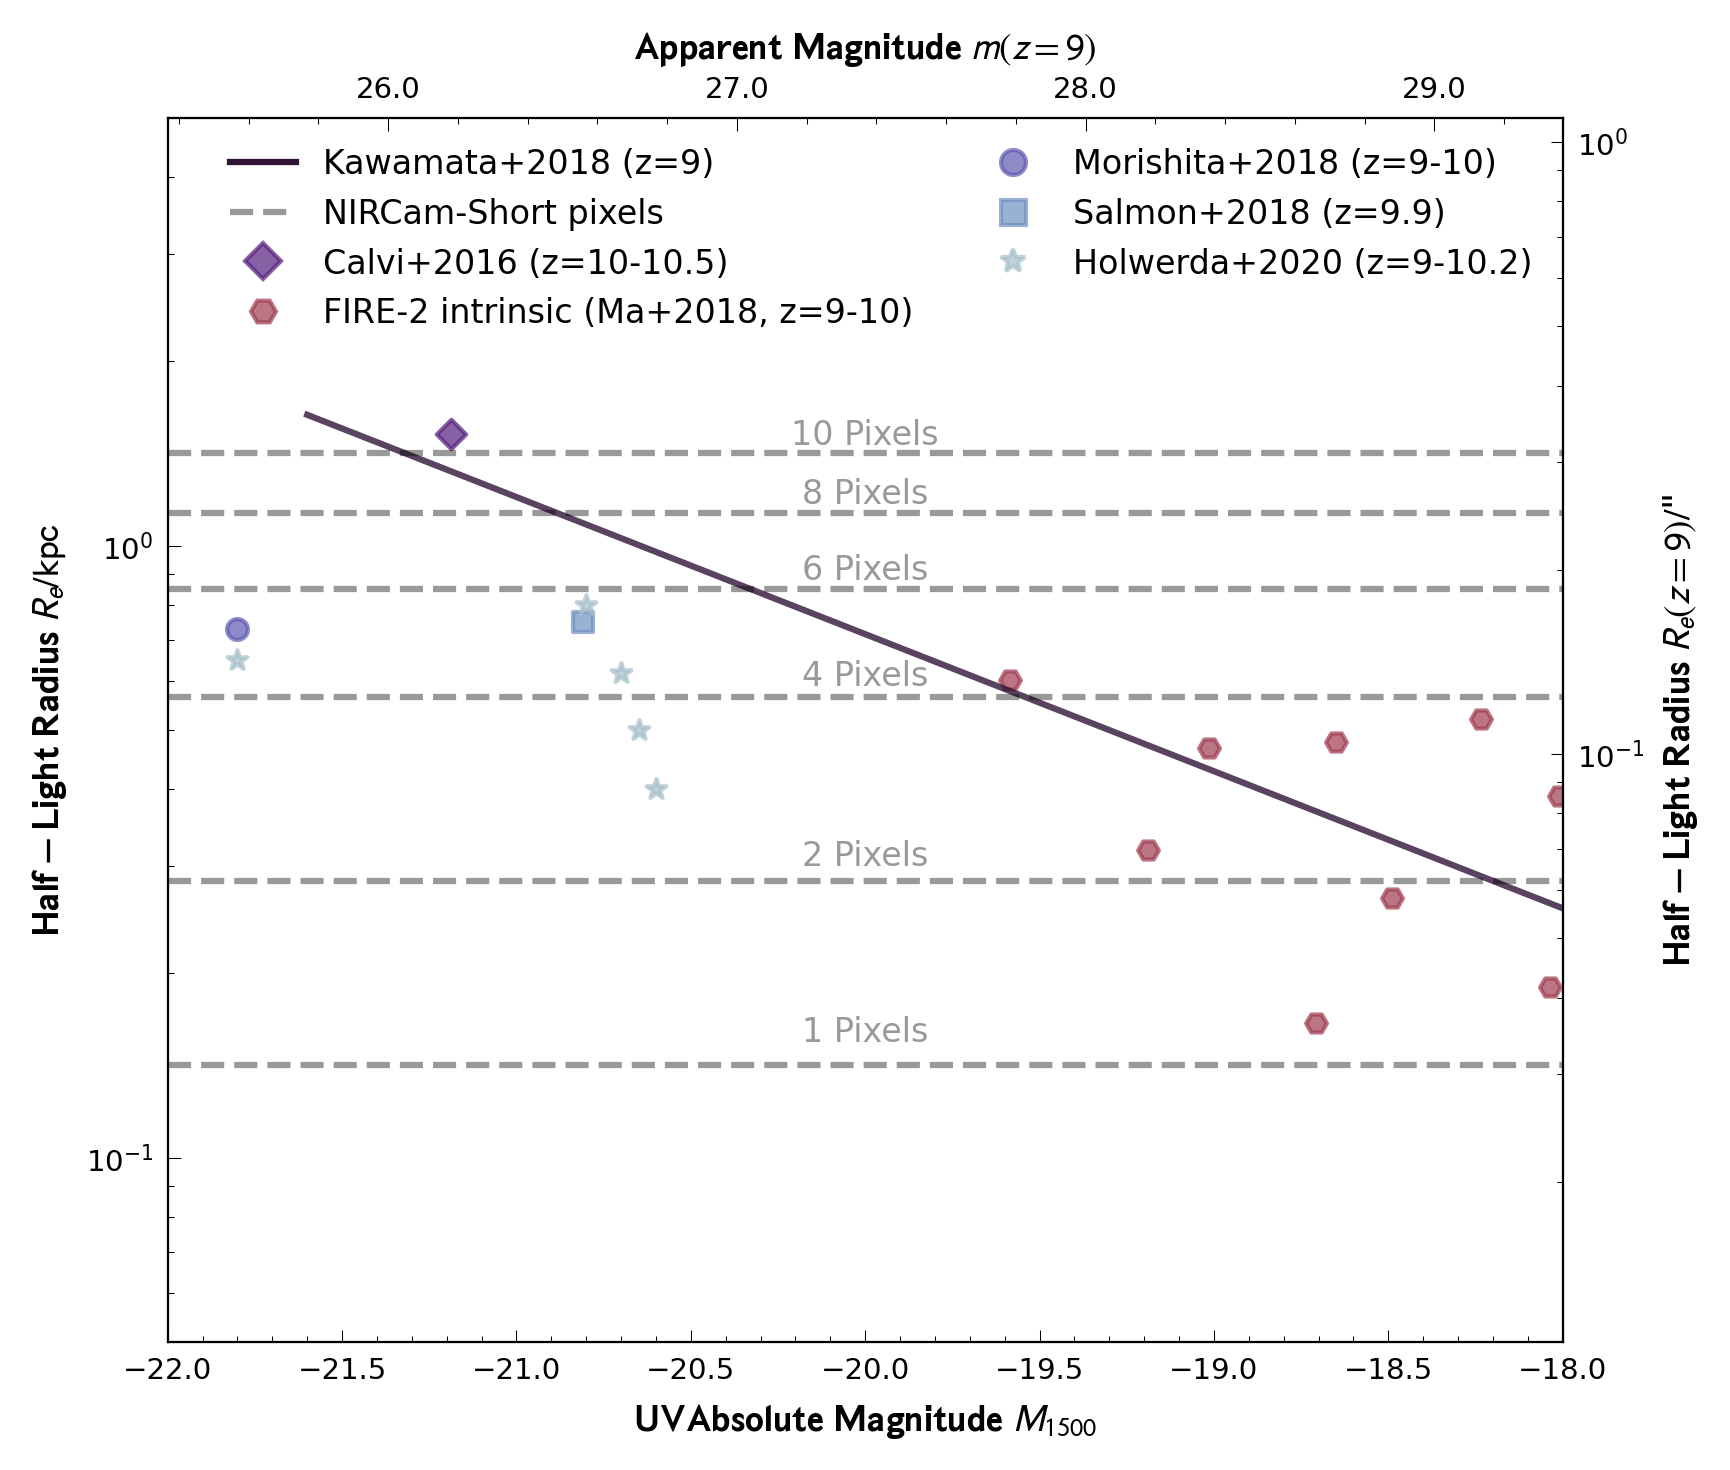
\includegraphics[width=0.6\textwidth]{figs/morph.png}
      \caption{\protect\rule{0ex}{10ex} Current observation constraints and theoretical predictions for the sizes of galaxies at $z>9$. \textbf{Even in under-sampled imaging many $z>9$ galaxies are expected to be resolved in the NIRCam imaging.}}
      \label{fig:sizes}
\end{SCfigure}


\subsection*{Legacy science}

{\bf could add quiescent galaxies at $z>3$ here}

{\bf -- similar to WAFLS --}

{\bf faint late-type stars}

{\bf faint lower redshift galaxies -- photo-z, physical properties, morphologies}

{\bf follow-up studies}




%%%%%%%%%%%%%%%%%%%%%%%%%%%%%%%%%%%%%%%%%%%%%%%%%%%%%%%%%%%%%%%%%%%%%%%%%%%

%   2. TECHNICAL JUSTIFICATION
%       (see https://jwst-docs.stsci.edu/jwst-opportunities-and-policies/jwst-call-for-proposals-for-cycle-1/jwst-cycle-1-proposal-preparation)
%
%

\clearpage

\justifyobservations   % Do not delete this command.
% Enter your description of the observations.

\noindent
\underline{\bf Filter choice: photometric redshifts -- } Simulations show that the combination of 3 filter pairs: {\bf F115W}, {\bf F150W}, {\bf F200W}, {\bf F277W}, {\bf F356W}, and {\bf F444W} is the optimum choice for \emph{robustly} identifying $z>9$ star forming galaxies. 2 pairs can in principle be used to detect galaxies $9<z<11$ however the contamination rate is higher and the accuracy/precision at $z>11$ drops significantly. 2 pairs also limits the extent to which the UV continuum slope $\beta$ can be measured \emph{consistently} across redshifts. Adding {\bf F090W} has little effect on the the reliability of the redshifts of galaxies at $z>9$ though does extend the redshift range down to $z\sim 7$ providing increased legacy science. While noting that 3 filter pair strategy best matches our scientific objectives these can be partially met or even \emph{exceeded} using a 2 or 4 pair strategy respectively. To keep PUPPIES as flexible as possible we can also make use of opportunities better suited to a 2 or 4 pair strategy though note a preference those opportunities amenable to our default scenario.


\underline{\bf Filter choice: physical properties -- } Constraining the chemical and dust enrichment of galaxies at $9<z<11$ requires that we probe the rest-frame UV continuum with at least a single colour, and ideally with several bands providing a consistent measurement of the same wavelength range across several redshifts. A 6-band strategy is ideal in this respect as it allows the UV continuum to probed with 3 bands uncontaminated by the Lyman-$\alpha$ and Balmer breaks, encompassing the entire rest-frame UV, across our entire target redshift range. 


\begin{SCfigure}
    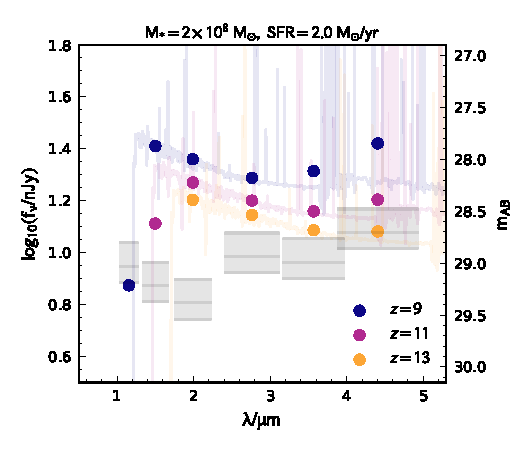
\includegraphics[width=0.6\textwidth]{figs/SED.pdf}
      \caption{\protect\rule{0ex}{10ex} The expected NIRCam fluxes of a $2\times 10^{8}\ {\rm M_{\odot}}$ star forming galaxies at $z=9$, $z=11$, and $z=13$. \todo{Very similar to WAFLS figure.}}
      \label{fig:SED}
\end{SCfigure}


As demonstrated using simulated galaxies in Figure \ref{fig:beta}, when combined with F444W the degeneracy of $\beta$ with these physical properties can be broken allowing the measurement of stellar masses, specific star formation rates, and dust attenuation. Measuring the dust attenuation not only allows us to account for obscured star formation but will also help constrain the mechanism(s) responsible for the assembly of the large observed reservoirs of dust in the early Universe.



\begin{figure}[h!]
    \centering
    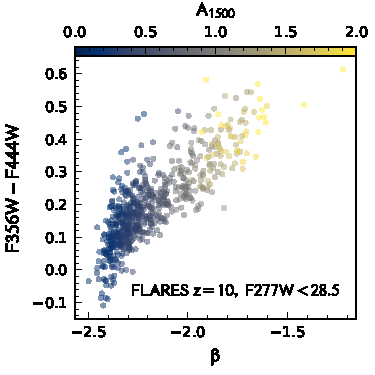
\includegraphics[width=0.45\textwidth]{figs/beta_A1500.pdf}
    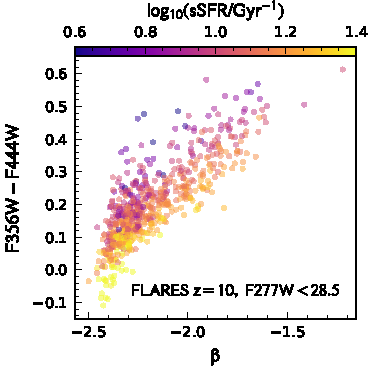
\includegraphics[width=0.45\textwidth]{figs/beta_sSFR.pdf}
    % 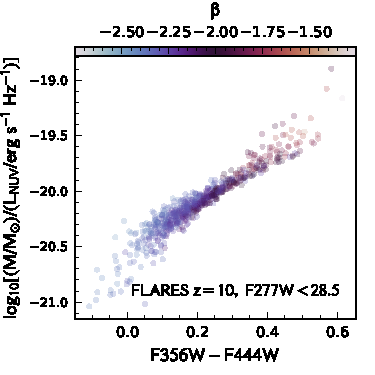
\includegraphics[width=0.3\textwidth]{figs/C_beta_MTOL.pdf}
    \caption{The relationship between $\beta$ and F356W-F444W for simulated galaxies at $z=10$ colour-coded by $A_{1500}$ (\emph{\underline{left}}) and specific star formation rate (\emph{\underline{right}}) predicted by the FLARES simulation (Lovell+2020; Vijayan+2020). At these redshifts $\beta$ is strongly correlated with dust attenuation while at fixed $\beta$ the specific SFR is correlated with F356W$-$F444W. \textbf{The 6 filter observations obtained by PUPPIES will enable us to measure the dust attenuation, total star formation rates, and stellar masses of galaxies at $z>8$.}}
    \label{fig:beta}
\end{figure}

\noindent
\underline{\bf Area and Depth:} PUPPIES is an opportunity led program: we are interested in obtaining deep NIRCam imaging in 10-20 independent pointings to complement the existing shallower, but wider, Cosmic Evolution Early Release Science (CEERS) survey. Compared to a similarly sized contiguous survey 10-20 independent sight-lines should reduce the cosmic variance contribution to the total variance by around $3-5$.

\noindent
To determine the type, and thus potential depth, of opportunities that are available we use the public GTO and ERS APTs and filter out all observations that 1) already have attached coordinated parallels, 2) have the \texttt{NoParallel} flag set, and 3) those of targets with high-background ($>0.3\ {\rm MJy/Sr}$). To estimate the amount of time available to teach unique target we sum the science durations of all observations using the same instrument. The predicted distribution of opportunities with science durations $t_{\rm SD}>10^{4}$ s is then shown in Figure \ref{fig:time_background}: this analysis suggests $\sim 50$ GTO/ERS opportunities with $t_{\rm SD}>10^{4}$ s; assuming this distribution is representative of the final Cycle 1 observation suggests there should be $100-150$ useful opportunities.

\begin{SCfigure}
    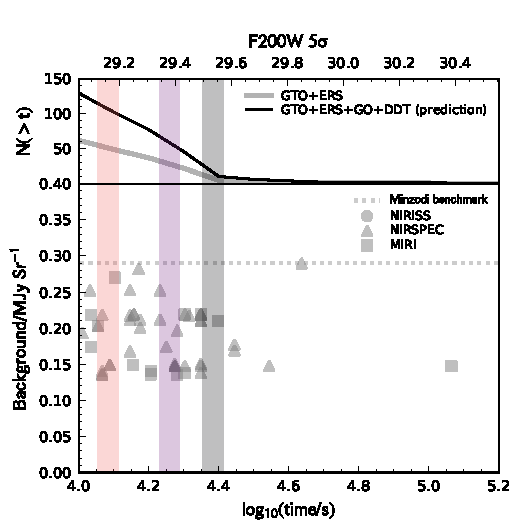
\includegraphics[width=0.6\textwidth]{figs/time_background.pdf}
      \caption{\protect\rule{0ex}{10ex} The predicted distribution of science durations $t_{\rm SD}$ and backgrounds for pure parallel observing opportunities based on the existing GTO and ERS programs. The vertical bands denote the 3 tiers used to define our fiducial survey while the horizontal lines denote the $2\mu$m \texttt{minzodi} benchmark background and the minimum background in several deep extragalactic fields. The top panel shows the resulting cumulative distribution of opportunities as well as an extrapolation to the full cycle 1 observations.}
      \label{fig:time_background}
\end{SCfigure}

\noindent
\underline{\bf Fiducial programme:} Armed with this predicted knowledge we define a fiducial programme consisting of three tiers - ABC - assuming 4, 3, and 2 \texttt{deep8} 10 group exposures respectively. Reflecting the greater availability of shorter duration opportunities we choose, for this fiducial programme, to obtain 3, 5, and 10 pointings for the A, B, and C tiers respectively. The resulting area and depths achieved in each tier are summarised below. \textbf{The total exposure time as reported by the APT for the combination of the 3 tiers is 79.3 hours}.

\begin{table}[h!]
\footnotesize
\begin{center}
\begin{tabular}{ |c|c|c|c|c|c|c|c|c| } 
\hline
\multicolumn{3}{|c|}{} & \multicolumn{6}{|c|}{$5\sigma$ point-source depth} \\
 \hline
Tier & $N_{p}$ & Area$/{\rm arcmin^2}$ & F115W & F150W & F200W & F277W & F356W & F444W \\
\hline
\textbf{A} & 3 & 27 & 29.19 & 29.37 & 29.54 & 29.09 & 29.15 & 28.86 \\
\textbf{B} & 5 & 45 & 29.03 & 29.22 & 29.38 & 28.94 & 28.99 & 28.70 \\
\textbf{C} & 10 & 91 & 28.81 & 28.99 & 29.16 & 28.71 & 28.77 & 28.48 \\
\hline
\end{tabular}
\end{center}
\vspace{-5mm}
\caption{The number of pointings $N_p$, area, and 5$\sigma$ point source depths in each filter for our 3 tiers for our fiducial survey.  Depths assume a short-wavelength (long-wavelength) apertures of $0.08$" ($0.16$"), background at the benchmark level of the \texttt{Minzodi} location as defined by \texttt{Pandeia}. The ABC tiers assume 4, 3, 2 exposures of 10 groups assuming the \texttt{DEEP8} readout mode respectively.}
\end{table}

\noindent
\underline{\bf Preferred distribution:} We would preferentially go deeper while keeping at least 10 independent sight-lines. 


\noindent
\underline{\bf Synergy with existing and planned surveys} PUPPIES will, partly through the expected availability of suitable parallel observing opportunities and partly through the primary scientific objectives, naturally complement planned programmes on \emph{Webb}, specifically CEERS and JADES. A comparison of the F150W, F200W, and F356W $5\sigma$ point-source depths and areas expected by WAFLS, CEERS, and JADES are shown in Figure \ref{fig:depth}. Figure \ref{fig:depth} also demonstrates the dramatic improvement of WAFLS over existing Hubble and Spitzer surveys. Compared to programmes reaching (surveying) a similar depth (area) on Hubble, WAFLS probes an approximately 10$\times$ larger area (1 magnitude deeper). There are no Spitzer surveys reaching a comparable depth in F356W/F444W with WAFLS reaching 2 magnitudes deeper than similar area surveys. By focusing on the $z>9$ Universe WAFLS will also complement the upcoming Euclid satellite which will be limited to $z\approx 8$. \todo{Needs updating}

\begin{SCfigure}
    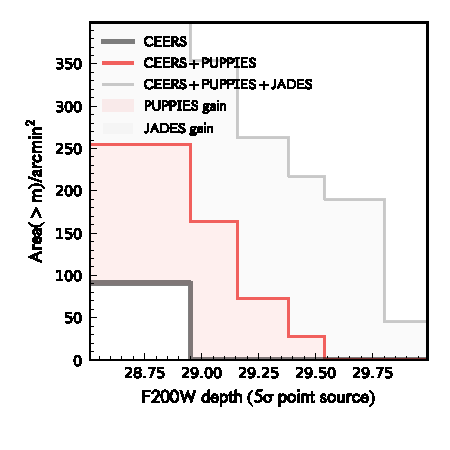
\includegraphics[width=0.6\textwidth]{figs/F200W.pdf}
      \caption{\protect\rule{0ex}{5ex} The cumulative area probed by PUPPIES, JADES, CEERS, and existing \emph{Hubble} and \emph{Spitzer} surveys as a function of the H/F150W-band, F200W, and $3.6\mu$m/F356W (right) depths. \todo{Which is better?}}
      \label{fig:depth}
\end{SCfigure}


\noindent
\underline{\bf Additional constraints} When selecting potential parallel slots we will not only consider potential science duration and background but also the availability of ancillary observations and accessibility to other facilities (e.g. ALMA).



%%%%%%%%%%%%%%%%%%%%%%%%%%%%%%%%%%%%%%%%%%%%%%%%%%%%%%%%%%%%%%%%%%%%%%%%%%%

%   3. SPECIAL REQUIREMENTS
%        (see https://jwst-docs.stsci.edu/jwst-opportunities-and-policies/jwst-call-for-proposals-for-cycle-1/jwst-cycle-1-proposal-preparation)
%
%
\specialreq             % Do not delete this command.
% Justify your special requirements here, if any.

%%%%%%%%%%%%%%%%%%%%%%%%%%%%%%%%%%%%%%%%%%%%%%%%%%%%%%%%%%%%%%%%%%%%%%%%%%%

%   4. COORDINATED PARALLEL OBSERVATIONS
%        (see https://jwst-docs.stsci.edu/jwst-opportunities-and-policies/jwst-call-for-proposals-for-cycle-1/jwst-cycle-1-proposal-preparation)
%
%
\coordinatedobs % Do not delete this command.
% Enter your coordinated parallel observing plans here, if any.

%%%%%%%%%%%%%%%%%%%%%%%%%%%%%%%%%%%%%%%%%%%%%%%%%%%%%%%%%%%%%%%%%%%%%%%%%%%

%   5. JUSTIFY DUPLICATIONS
%        (see https://jwst-docs.stsci.edu/jwst-opportunities-and-policies/jwst-call-for-proposals-for-cycle-1/jwst-cycle-1-proposal-preparation)
%
%
\duplications           % Do not delete this command.
% Enter your duplication justifications here, if any.

%%%%%%%%%%%%%%%%%%%%%%%%%%%%%%%%%%%%%%%%%%%%%%%%%%%%%%%%%%%%%%%%%%%%%%%%%%%

%   6. ANALYSIS PLAN
%       (see https://jwst-docs.stsci.edu/jwst-opportunities-and-policies/jwst-call-for-proposals-for-cycle-1/jwst-cycle-1-proposal-preparation)
%
%
\analysisplan % Do not delete this command.
% Describe the data processing and analysis plan here.

%%%%%%%%%%%%%%%%%%%%%%%%%%%%%%%%%%%%%%%%%%%%%%%%%%%%%%%%%%%%%%%%%%%%%%%%%%%

\clearpage

\bibliography{WAFLS,WAFLS_quiescent}


\end{document}          % End of proposal. Do not delete this line.
                        % Everything after this command is ignored.
